\documentclass[10pt]{article}
\usepackage{enumitem}
\usepackage{listings}
\usepackage{underscore}
\usepackage[ddmmyyyy]{datetime}
\renewcommand{\dateseparator}{--}
\usepackage[bookmarks=true]{hyperref}
\usepackage[utf8]{inputenc}
\usepackage[english]{babel}
\usepackage{url}
\usepackage{graphicx}

\newenvironment{enum}
{\begin{enumerate}[label*=\arabic*.][resume]}
{\end{enumerate}}

\hypersetup{
    pdftitle={Software Requirement Specification},    
    pdfauthor={Dakota Wessel},                     
    pdfsubject={TeX and LaTeX},                        
    pdfkeywords={TeX, LaTeX, graphics, images}, 
    colorlinks=true,       
    linkcolor=blue,       
    citecolor=black,       
    filecolor=black,        
    urlcolor=purple,        
    linktoc=page            
}
\def\myversion{1.0.0}
\date{}
\usepackage{hyperref}
\begin{document}

\begin{flushright}
    \rule{16cm}{5pt}\vskip1cm
    \begin{bfseries}
        \Huge{SOFTWARE REQUIREMENTS\\ SPECIFICATION}\\
        \vspace{1.0cm}
        for\\
        \vspace{1.0cm}
        Checkers\\
        \vspace{1.5cm}
        \LARGE{Version \myversion}\\
        \vspace{1.5cm}
        Prepared by:\\
    Adam Luong\\
    Benny Mai\\
    Dakota Wessel\\
    Jacky Zheng\\
    Tony Zhu\\
        \vspace{1.9cm}
        Group: \textbf{10}\\
        \vspace{1cm}
        \today\\
    \end{bfseries}
\end{flushright}

\tableofcontents

\section*{Revision History}

\begin{center}
    \begin{tabular}{|c|c|c|c|}
        \hline
        Name & Date & Reason For Changes & Version\\
        \hline
        1.0.0 & \formatdate{15}{10}{20} & Initial Setup & Dakota Wessel\\
        \hline
    \end{tabular}
\end{center}

\section{Introduction}

\subsection{Purpose of Document}
The goal of this document is to outline the requirement specifications of our web-based checkers game. 
This application will allow two users to connect and interact remotely, allowing them to play and chat. 
This document will cover the scope, objective, basic requirements, and goals for this application. 
After the application's high-level look, this document will dive deeper into topics like functional, 
non-functional, user interface, design, test cases, program usage, and references. 
This document will clearly explain to an engineer or end-user the overall implementation 
and goals of our application.

\subsection{Project Scope}
The main objective for documentation is to educate the reader about our Checkers application, 
its functionality, the technologies used, and outline the application requirements.

\subsection{Overview of Document}
The documentation will provide a clear explanation about which technologies we used, 
how we implemented them, and why we chose to use them. It will outline each component 
of our application. The flow starts with the functional requirements, non-functional requirements, 
user interface, and finished with lobbies, gameplay, and winning conditions, concluding with our references. 

\subsection{Background}

\subsubsection{History}

Throughout history, the game Checkers has been around, so the exact date for Checkers' 
invention is unknown. One of the earliest records of the game dates back to 3000 B.C in what 
is present-day Iraq. Later in Egypt, in 1400 B.C, the game was played using a 5 x 5 board \cite{historyCheckers}. 
However, the version of Checkers that we know of today was established in the mid-1500s by an English mathematician. 
Now the board game of checkers is cemented as one of the most popular board games of all time. 
\subsubsection{Game Rules}
    The rules provided are from the American Checker Federation \cite {checkersFoundation}.
    \begin{enumerate}
    \item Red always makes the first move.
    \item A player can forfeit at any time; as a result, the opponent wins.
    \end{enumerate}
\subsubsection{Moves} 
\begin{enumerate}
    \item A player may only move their own pieces.
    \item Normal Piece
        \subitem A normal piece may only move toward the other player's side of the board.
        \subitem A normal piece may move diagonally to the left or right to a vacant square in front of it.
        \subitem A normal piece may capture on the diagonal if there exists a vacant square one more diagonal position ahead.
            \subsubitem A piece may move again if there exists another piece to capture after making a capture.
    \item A King Piece moves the same as a normal piece but can move and capture backward.
    \item A King Piece may capture forward or backward.
    \item If a normal piece reaches the opposite edge of the board, it becomes a King Piece.
\end{enumerate}   

\subsubsection{Win Condition}
\begin{enumerate}
    \item When one player has no more pieces to move, the other player is the winner.
    \item If a player forfeits the match, the other player is conceded the winner.
\end{enumerate}

\subsection{Abstract}

Our goal is to create a document that will help a team member create an application, 
both client-side and server-side, that allows remote users to play checkers. The construction of this application will host one game of checkers to two users. 
\section{Overall Description}

\subsection{Product Functions}

\begin{enumerate}
    \item Provide an application to host a checkers game with two user over the local network or internet.
    \item Provide a server that mediates gameplay, game sessions, and client interactions.
\end{enumerate}

\subsection{Assumptions and Dependencies}

\begin{enumerate}
    \item A connection to a local network or internet connection.
    \item A computer with a graphical environment for the client
    \item A Unix or Windows based server.
    \item Knowledge of the rules of checkers.
    \item Client know how to launch a python file.
\end{enumerate}

\section{Functional Requirements}

\subsection{Client}

\begin{enumerate}[label*=R\arabic*.]
    \item Client - Server Interaction
    \begin{enumerate}[label*=\arabic*.]
        \item Clients will be able to request a new game session from the server and be given a unique ID from the server.
        \item Clients will be able to connect to an existing game session by providing an unique ID to the server.
        \item Clients will not be able to connect to a game session with an incorrect unique ID.
        \item Clients will be able to pause a game session given approval from both clients.
        \item Clients will be able to leave from the game session without consequence should the game be paused.
        \item Clients will be able to leave from the game session regardless of game state other than paused, but will immediately concede the game.
    \end{enumerate}
\end{enumerate}

\subsubsection{Board State}

\begin{enumerate}[resume*]
    \item Board
    \begin{enumerate}[label*=\arabic*.]
        \item The clients will have a copy of the board for rendering purposes
        \item The board will update upon receiving a server update
    \end{enumerate}
\end{enumerate}

\subsection{Server}

\begin{enumerate}[resume*]
    \item Server status
    \begin{enumerate}[label*=\arabic*.]
        \item Server should be able to be run constantly without crashing.
        \item Server will have a heartbeat function that will send an email to the developers if the server is down.
    \end{enumerate}
    \item Server - Client Interaction
    \begin{enumerate}[label*=\arabic*.]
        \item Server will be able to process client connection information to create a lobby.
        \item Server will keep track of clients and game sessions.
        \item Server will keep track of time clients have spent on each move.
            \subitem Should a client go over specified time limit, initiate game loss state for that client.
        
        \item On user timeout, wait a set amount of time.
            \subitem If not connected within that time, signal other client game has ended due to disconnected player.
        \item Server will validate moves before sending updated move to clients.
            \subitem On invalid move, signal client that move was invalid and to try again.
    \end{enumerate}
    \item Server - Lobby Interaction
    \begin{enumerate}[label*=\arabic*.]
        \item Server will first check that a port is open before assigning it to a lobby upon creation.
        \item Server will close the port assigned to a lobby when the game has been finished.
    \end{enumerate}
\end{enumerate}

\section{Other Requirements}

\subsection{System Requirements}

\begin{enumerate}[label*=S\arabic*.]
    \item Server and Client
        \subitem Python3
    \item Client
        \subitem Windowing display environment:
            \subsubitem Windows
            \subsubitem MacOS
\end{enumerate}

\subsection{Network Requirements}

\begin{enumerate}[label*=N\arabic*.]
    \item Client and Server
	 \begin{enumerate}[label*=\arabic*.]
        \item An active internet connection
        \item port forwarding configured properly on their local network
        \item Client must be connected to Drexel's network
        \item Response time to the server must be less than 120ms
	  \end{enumerate}
    \item Server
 	\begin{enumerate}[label*=\arabic*.]
        \item Server must be hosted on tux.cci.drexel.edu
        \item Server will be running on one dedicated box
  \end{enumerate}
\end{enumerate}

\section{User Interface}

\subsection{Framework}

The project shall use Python3? to create the user interface.

\subsection{Menus}

\begin{itemize}
\item Main Menu
    \subitem Play Game button: connects player to the server
    \subitem Quit Game: closes the game

\item Game Lobby
    \subitem Show players in the lobby
    \subitem Ready? button: start game once both players click
    \subitem Main Menu button: return to the main menu

\item Game
    \subitem Checkers match screen, showing a checkers board with both players’ pieces
        \subsubitem Player’s “side” of the board is always on the bottom of the screen
    \subitem Top of screen shows whose turn it is: Black or Red
        \subsubitem During the player’s turn, they click on a piece to select it
        \subsubitem Piece becomes highlighted, as does all valid spaces the player could move to
        \subsubitem Player clicks on a highlighted space to move the piece there or clicks on a new piece to select it
        \subsubitem After a move has been made, the game checks if there is a winner. Move to Winner Display if a winner is found. Otherwise, start next player’s turn.

\item Winner Display
    \subitem Show the player who won the game: Black or Red
    \subitem Rematch? No button: return both players to the main menu
    \subitem Rematch? Yes button: register this player as wanting a rematch
        \subsubitem If both players click Yes, then return both players to the Game Lobby screen
\end{itemize}

\section{Standard Components}

\begin{itemize}
    \item Buttons: used for menu interations and navigation.
    \item Pieces: The pieces will be the basic playing pieces within gameplay.
    \item King Pieces: These pieces will behave identically to the regular pieces, but with additional movement options according to the rules of Checkers.
    \item Checkers Board: an 8x8 grid of alternating black and red tiles on which all pieces will be displayed in the gameplay.
\end{itemize}

\subsection{Program Usage}
\subsubsection{Gameplay}
\begin{enumerate}[label*=G\arabic*.]
	\item The match begins with an 8x8 grid with each tile alternating between black and red in color.
	\item One player is assigned the black pieces and the other red.
	\item Each player’s pieces start on opposite ends of the board, occupying every other space within the first three rows (for a total of 12 pieces for each player).
	\subitem See attached image for an example checkers setup:
	\subitem 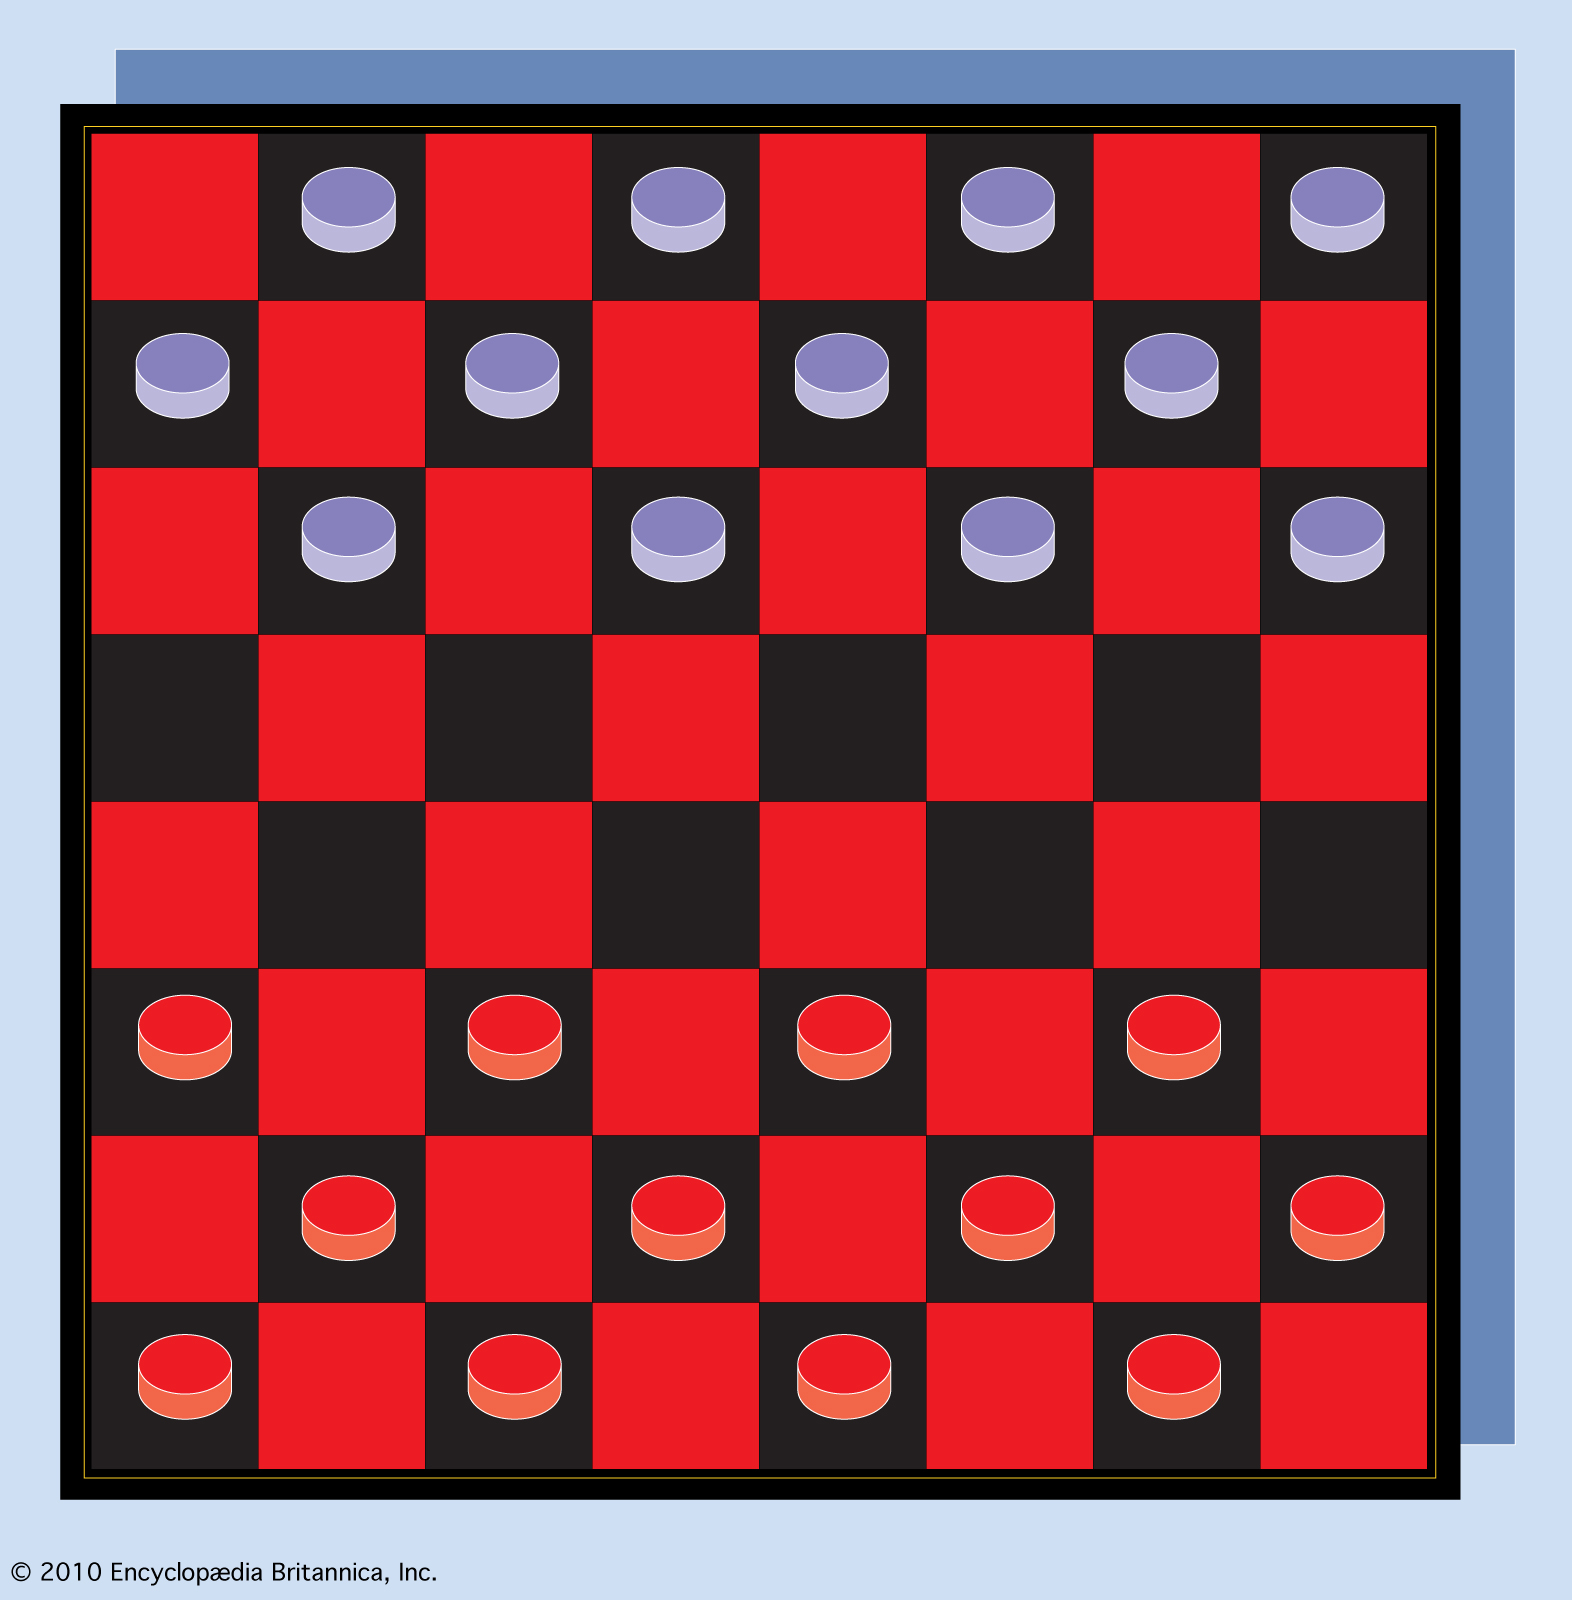
\includegraphics[width=8cm]{board.png}
	\item The black player starts the match by taking their turn.
	\item During each turn, the active player selects a piece of their own to move according to the following rules:
\begin{itemize}
    \item If the piece is bordering an enemy piece and there is a free space on the other side of that enemy piece, the piece must “jump” to the empty space, removing the enemy piece it moved over from the board
        \subitem Multiple jumps can be made in a single turn if the piece is in position to jump an additional enemy piece after completing a jump
    \item If the piece cannot jump, it may move diagonally one space to an unoccupied space
        \subitem If the piece is a non-king, it must move forward
        \subitem If the piece is a king, it can move in any direction
    \item A piece cannot jump over pieces of the same color as itself (friendly pieces)
    \item Two pieces cannot occupy the same space, regardless of color
\end{itemize}

\item When a non-king piece has reached the edge of the board opposite its color’s starting side, that piece will be crowned and turned into a king, allowing it to move in any direction.
\end{enumerate}
\subsubsection{Win Conditions}

\begin{enumerate}
    \item If player A has no more pieces, player B is the winner and vice versa.
    \item If player A disconnects, player B is the winner and vice versa.
\end{enumerate}


\begin{thebibliography}{9}

\bibitem{checkersFoundation}
  The American Checker Foundation,
  \textit{USA Checkers},
  https://www.usacheckers.com/,
  2019.

\bibitem{historyCheckers}
W.J. Rayment,
\textit{History of Checkers or Draughts},
http://www.indepthinfo.com/checkers/history.shtml,
2004.

\end{thebibliography}


\end{document}